\documentclass[sagev]{sagej}

\usepackage{graphicx}
\usepackage{amsmath,amssymb,bm}
\usepackage{booktabs}
\usepackage{hyperref}
\usepackage{color}

% ------- numbers still to be filled from benchmark/results (marked in red) ----
\newcommand{\TODOnum}[1]{\textcolor{red}{[#1]}}

\def\volumeyear{2026}

\begin{document}

\runninghead{Bachrathy}

\title{Higher-Order Multiplication-Free Stability Analysis of Time-Periodic
Delayed Systems: Runge--Kutta and Collocation Steps and the
Accuracy--Sparsity Trade-off}

\author{D\'aniel Bachrathy\affilnum{1}}

\affiliation{\affilnum{1}Department of Applied Mechanics, Faculty of Mechanical
Engineering, Budapest University of Technology and Economics, Budapest, Hungary}

\corrauth{D\'aniel Bachrathy, Department of Applied Mechanics, Budapest
University of Technology and Economics, M\H{u}egyetem rkp.~3., H-1111
Budapest, Hungary.}

\email{bachrathy@mm.bme.hu}

\begin{abstract}
The multiplication-free semi-discretization method (MFSD) reduces the
stability analysis of time-periodic delay differential equations to a sparse,
banded generalized eigenvalue problem with linear time complexity in the
resolution $p$; however, the classical piecewise-constant step limits its
convergence order to two. This paper shows that, once the analysis is written
in the multiplication-free form, the per-step integrator becomes a free design
choice: the residual block rows of any explicit Runge--Kutta or implicit
collocation scheme (Gauss--Legendre, Radau, Lobatto) can be embedded in the
banded system through their Butcher tableaux, raising the convergence order of
the dominant characteristic multipliers to the order of the chosen scheme ---
super-convergent order $2s$ for $s$-stage Gauss collocation --- provided the
delayed terms are interpolated by the continuous extension of the same scheme.
In the limit of a single ultra-high-order step, the framework degenerates to
the known global collocation (pseudospectral) method; between the two extremes
lies a continuum in which per-step order is traded against matrix sparsity.
Because the number of nonzeros grows cubically with the stage number while the
error decreases only exponentially, the CPU-time optimum for a prescribed
accuracy is a problem-dependent \emph{sweet spot} at moderate order and many
steps, which we locate experimentally for a small benchmark system (the
delayed Mathieu equation) and a high-dimensional finite-element beam with
delayed boundary feedback. We further argue that previous
``collocation versus semi-discretization'' comparisons conflated
$p$-refinement with $h$-refinement, and we prescribe a fair work--precision
methodology (log--log axes, wide resolution ranges, variance-reported CPU
times, one machine and thread configuration). All methods are released in the
open-source Julia package \textsf{MFCM.jl}.
\end{abstract}

\keywords{Time-delay systems, semi-discretization, collocation, Runge--Kutta
methods, Floquet theory, stability analysis, computational complexity}

\maketitle

\section{Introduction}
\label{sec:intro}

Time-periodic linear delay differential equations (DDEs) of the form
\begin{equation}
  \dot{\mathbf{x}}(t) = \mathbf{A}(t)\,\mathbf{x}(t)
    + \sum_{k=1}^{g}\mathbf{B}_k(t)\,\mathbf{x}\bigl(t-\tau_k(t)\bigr)
    + \mathbf{c}(t),
  \label{eq:ldde}
\end{equation}
with $T$-periodic coefficients $\mathbf{A}(t)$, $\mathbf{B}_k(t)$, delays
$\tau_k(t)$ and forcing $\mathbf{c}(t)$, govern a wide range of engineering
and biological systems: regenerative machine-tool chatter
\citep{Tobias1965,Altintas2012,Munoa2016}, turning with spindle-speed
variation \citep{Long2007,Seguy2008}, feedback control with latency
\citep{Stepan1989}, and seasonally forced population dynamics. Their
asymptotic stability is decided by the dominant characteristic multipliers of
the monodromy operator associated with one period \citep{Insperger2011}.

Two families of numerical methods dominate practice. Semi-discretization (SD)
\citep{Insperger2002,Insperger2011} advances the state with a fixed step
$\Delta t = T/p$, treating the delayed term (and, in the classical zeroth- and
first-order variants, the coefficients) as piecewise constant or piecewise
linear per step; its convergence order is limited to two
\citep{Insperger2008}. Collocation and pseudospectral methods
\citep{Breda2005,Breda2015} represent the solution segment by a global
high-order polynomial and converge spectrally for smooth problems. A
recurring claim in the literature is that collocation ``outperforms''
semi-discretization; we argue in Section~\ref{sec:fair} that such comparisons
are structurally unfair, because they compare a $p$-refinement strategy
(raising the polynomial order) with an $h$-refinement strategy (shrinking the
step) --- the same category error as declaring $p$-type finite elements
universally superior to $h$-type ones.

The recent multiplication-free semi-discretization method (MFSD)
\citep{Bachrathy2026} removed the main cost bottleneck of SD: instead of
multiplying $p$ one-step matrices into a dense monodromy matrix
($\mathcal{O}(p^{2.8})$ in practice), every step is written as a residual
equation and all $p$ steps are stacked into one sparse banded system, whose
one-period transition is obtained from the generalized eigenvalue problem
$\mathbf{\Phi}_\mathrm{L}\mathbf{y}_p = \mathbf{\Phi}_\mathrm{R}\mathbf{y}_0$
at $\mathcal{O}(p)$ cost. The MFSD assembly is inherited machinery here and is
\emph{not} claimed as a contribution of the present paper.

The present paper starts from a simple observation: \emph{the
multiplication-free form only needs a per-step residual}. Semi-discretization
is, structurally, a fixed-step time integrator whose only approximation is the
per-step treatment of the coefficients and the delayed term. Consequently, the
piecewise-constant step can be replaced by \emph{any} one-step scheme --- an
explicit Runge--Kutta method or an implicit collocation method --- by placing
the Butcher-tableau coefficients into the residual block rows and augmenting
the per-step state with the internal stage values. This raises the achievable
convergence order arbitrarily, at a quantifiable structural price: the sparse
matrices become denser as the stage number grows.

The contributions are, honestly delimited:
\begin{enumerate}
  \item the systematic embedding of arbitrary Runge--Kutta and collocation
        steps (via their Butcher tableaux and continuous extensions) into the
        multiplication-free banded stability framework for time-periodic
        DDEs, including time-periodic delays (Section~\ref{sec:method});
  \item the explicit-versus-implicit matrix-structure and CPU trade-off
        analysis, and the demonstration that the single-step limit reproduces
        the known global collocation method (Section~\ref{sec:spectral});
  \item the identification and characterization of the accuracy--sparsity
        \emph{sweet spot}: for a given accuracy target the CPU optimum lies
        at moderate per-step order and many steps, at a location that depends
        on the problem dimension and resolution demand
        (Section~\ref{sec:results});
  \item a fair-comparison methodology that separates $p$- and $h$-refinement
        and reports work--precision curves with variance on one fixed
        machine configuration (Section~\ref{sec:fair}); and
  \item an open-source Julia implementation, \textsf{MFCM.jl}, with all
        scripts needed to reproduce every figure.
\end{enumerate}
Neither collocation itself \citep{Breda2005} nor the multiplication-free
assembly \citep{Bachrathy2026} is claimed as new; the value of the paper is
the unifying embedding, the trade-off quantification, and the practical
guidance it yields.

\section{Background: MFSD and semi-discretization as fixed-step integration}
\label{sec:background}

Discretize one principal period into $p$ uniform steps,
$\Delta t = T/p$, $t_n = n\,\Delta t$, and let
$r = \lceil \tau_{\max}/\Delta t\rceil$ count the steps covering the largest
delay. Classical SD constructs a one-step mapping
$\mathbf{x}_{n+1} = \mathbf{P}_n \mathbf{x}_n + \mathbf{R}_n
\mathbf{x}_{n-r}$ from the exact solution of the frozen-coefficient system
over $[t_n, t_{n+1}]$ \citep{Insperger2011}. The monodromy matrix is the
product of $p$ such mappings acting on the discretized history
$\mathbf{y}_n = (\mathbf{x}_n^\top,\ldots,\mathbf{x}_{n-r}^\top)^\top$;
forming this product costs $\mathcal{O}(p\,(rd)^\omega/r^\omega)$-ish work in
practice ($\approx\mathcal{O}(p^{2.8})$ measured in \citealp{Bachrathy2026}),
and its avoidance is the point of MFSD: each step contributes the residual
row $\mathbf{0} = \mathbf{I}\mathbf{x}_{n+1} - \mathbf{P}_n\mathbf{x}_n -
\mathbf{R}_n\mathbf{x}_{n-r}$ to a sparse banded block system over the
extended vector spanning $[t-\tau_{\max},\, t+T]$, split into left/right
blocks so that the spectrum follows from
$\mathbf{\Phi}_\mathrm{L}\mathbf{y}_p =
\mu\,\mathbf{\Phi}_\mathrm{R}\mathbf{y}_0$
via sparse Krylov iteration \citep{Saad1986,Haegeman2021} at
$\mathcal{O}(p)$ total cost \citep{Bachrathy2026}.

Two properties of this construction matter for what follows. First, the
one-step map is a \emph{fixed-step integrator}: the only approximation is
that $\mathbf{A}(t)$, $\mathbf{B}(t)$ and the delayed argument are frozen (or
low-order interpolated) across $\Delta t$. It is exactly this per-step
treatment that caps the convergence order at two: as shown by
\citet{Insperger2008}, a first-order approximation of the delayed term is
already optimal for the piecewise-constant coefficient scheme, and no
refinement of the classical SD step exceeds order two. Second, the assembly
touches the integrator only through the per-step residual; nothing in the
banded structure, the left/right splitting for $p-1 \gtrless r$, or the
Krylov solver depends on \emph{which} integrator produced the residual. The
integrator is a free design choice --- the theme of this paper.

\section{Higher-order multiplication-free stepping}
\label{sec:method}

\subsection{Stage-augmented residual blocks from a Butcher tableau}
\label{sec:butcher}

Consider an $s$-stage Runge--Kutta method with tableau
$(\mathbf{a}, \mathbf{b}, \mathbf{c})$, $a_{ij},\,b_j,\,c_j$,
applied to \eqref{eq:ldde} on $[t_n, t_n + \Delta t]$. Writing the stage
\emph{values} $\mathbf{Y}_{i}\approx\mathbf{x}(t_n + c_i\Delta t)$ (rather
than stage slopes), the step reads
\begin{align}
  \mathbf{Y}_i &= \mathbf{x}_n + \Delta t \sum_{j=1}^{s} a_{ij}
      \Bigl[\mathbf{A}(t_{nj})\,\mathbf{Y}_j + \mathbf{d}_j\Bigr],
      \qquad i = 1,\ldots,s,
  \label{eq:stage}\\
  \mathbf{x}_{n+1} &= \mathbf{x}_n + \Delta t \sum_{j=1}^{s} b_{j}
      \Bigl[\mathbf{A}(t_{nj})\,\mathbf{Y}_j + \mathbf{d}_j\Bigr],
  \label{eq:update}
\end{align}
with $t_{nj} = t_n + c_j \Delta t$ and the delayed-plus-forcing terms
\begin{equation}
  \mathbf{d}_j = \sum_{k=1}^{g} \mathbf{B}_k(t_{nj})\,
      \tilde{\mathbf{x}}\bigl(t_{nj} - \tau_k(t_{nj})\bigr) + \mathbf{c}(t_{nj}),
  \label{eq:delayterm}
\end{equation}
where $\tilde{\mathbf{x}}$ denotes the interpolated delayed state
(Section~\ref{sec:delayinterp}). The per-step unknown block is the
stage-augmented vector
\begin{equation}
  \mathbf{v}_n = \bigl(\mathbf{x}_n^\top,\,
    \mathbf{Y}_{1}^\top,\ldots,\mathbf{Y}_{s}^\top\bigr)^\top
    \in \mathbb{R}^{(s+1)d},
\end{equation}
and the global unknown $\mathbf{q} = (\mathbf{v}_1^\top,\ldots,
\mathbf{v}_p^\top)^\top$ collects all steps of one period. Equations
\eqref{eq:stage}--\eqref{eq:update} are linear in the current and delayed
states, so each step contributes one block row to a sparse system
$\mathbf{\Phi}_\mathrm{L}\,\mathbf{q} = \mathbf{\Phi}_\mathrm{R}\,
\mathbf{q}_\mathrm{hist}$, exactly as in MFSD but with $(s+1)d$-sized blocks:
the block bandwidth grows linearly and the per-block fill quadratically with
the stage number.

In the implementation the stage equations \eqref{eq:stage} are
\emph{pre-eliminated} per step: the stage-coupling matrix
$\mathbf{M}_n = \mathbf{I} - \Delta t\,(\mathbf{a}\otimes\mathbf{I}_d)\,
\mathrm{diag}\bigl(\mathbf{A}(t_{n1}),\ldots,\mathbf{A}(t_{ns})\bigr)$
of size $sd\times sd$ is factorized once (LU; a dense inverse for small
$sd$), and the responses of $(\mathbf{x}_{n+1}, \mathbf{Y}_1,\ldots,
\mathbf{Y}_s)$ to (i) $\mathbf{x}_n$, (ii) each delayed-state sample, and
(iii) the additive forcing are precomputed as $(s+1)d\times d$ transition
blocks. This keeps $\mathbf{\Phi}_\mathrm{L}$ \emph{unit block-lower
triangular} --- its LU factorization is trivial and fill-free --- while the
per-step elimination costs $\mathcal{O}\bigl(p\,(sd)^3\bigr)$, linear in $p$.
For explicit tableaux (strictly lower-triangular $\mathbf{a}$) the
elimination degenerates to forward substitution; for implicit collocation
tableaux (Gauss--Legendre of order $2s$, Radau~IIA of order $2s-1$,
Lobatto~IIIA of order $2s-2$ \citep{HairerWanner1996,Butcher2016}) it is a
genuine dense solve, which is precisely where the super-convergent order is
purchased.

\subsection{Delay interpolation by continuous extension}
\label{sec:delayinterp}

The delayed argument $t_{nj} - \tau_k(t_{nj})$ generally falls between grid
nodes, inside some earlier step $m$. Interpolating the delayed state with an
order lower than the integrator silently caps the observed convergence order
--- the higher-order analogue of the remark of \citet{Insperger2008} for the
classical scheme, and a classical result of DDE numerics
\citep{BellenZennaro2003}. The consistent choice is the \emph{continuous
extension} of the step itself: for collocation methods, the collocation
polynomial through $\bigl(\mathbf{x}_m, \mathbf{Y}_{1,m},\ldots,
\mathbf{Y}_{s,m}, \mathbf{x}_{m+1}\bigr)$ evaluated at the fractional
position $\theta \in [0,1]$ of the delayed instant inside step $m$; for
explicit methods, the scheme's dense-output polynomial (for RK4 the classical
cubic Hermite-type formula). The interpolation weights depend only on
$\theta$ and the tableau, so they join the precomputed transition blocks
without changing the banded structure; each delayed sample couples block row
$n$ to the two neighbouring history blocks $m$ and $m+1$. Since the
delayed state lies at least one full delay in the past, these couplings stay
strictly below the diagonal and $\mathbf{\Phi}_\mathrm{L}$ remains
triangular; couplings reaching into the pre-period history enter
$\mathbf{\Phi}_\mathrm{R}$ instead. Time-periodic delays $\tau_k(t)$ are
handled naturally, because $\theta$ and the target block $m$ are evaluated
per stage from $\tau_k(t_{nj})$.

\subsection{The single-step limit is global collocation}
\label{sec:spectral}

Setting $p = 1$ with an $s$-stage Gauss tableau makes the single step span
the entire period: the stage values \emph{are} then the collocation samples
of a global polynomial, and the construction reproduces the known
collocation/pseudospectral method for DDEs \citep{Breda2005,Breda2015} in its
strong form. This extreme is explicitly \emph{not} new; we include it (i) to
make the equivalence concrete --- in Section~\ref{sec:results} the
single-step spectrum matches the converged reference to near machine
precision --- and (ii) to expose its cost: the single-step matrix is
effectively dense, and the number of nonzeros of the assembled system grows
as $\mathcal{O}(d^2 s^3)$ with the stage count, so pushing all accuracy into
one step abandons exactly the sparsity that makes the multiplication-free
form fast. The continuum between ``$p$ large, $s$ small'' and ``$p=1$, $s$
large'' is the design space this paper maps.

\section{Fair-comparison methodology}
\label{sec:fair}

Comparisons between DDE stability methods frequently pit a $p$-refinement
method (collocation at increasing polynomial order) against an $h$-refinement
method (semi-discretization at decreasing step size) and report accuracy at a
single, often low, resolution on linear axes. Such comparisons cannot
identify asymptotic rates, hide constant factors, and --- like comparing
$p$-type against $h$-type FEM refinement --- do not license a universal
winner. The predecessor paper \citep{Bachrathy2026} already criticized
sub-100-resolution, non-log-log comparisons; we extend that critique into a
positive prescription:

\begin{enumerate}
  \item \textbf{Work--precision axes.} The primary comparison is CPU time
        versus eigenvalue error, both logarithmic, over wide ranges; the
        secondary one is CPU time versus resolution $p$ with fitted scaling
        exponents.
  \item \textbf{Variance-reported timing.} Every timed point is a warm-started
        mean over repeated runs with its standard deviation.
  \item \textbf{Both refinement families on the same axes.} Every method is
        shown under $h$-refinement, and the per-step order $s$ is swept
        separately (Section~\ref{sec:sweetspot}) so the full
        $(p,s)$-surface is visible, not a single slice.
  \item \textbf{Fixed environment.} One machine, one BLAS thread
        configuration, pinned package versions, deterministic start vectors;
        all reported alongside the results.
  \item \textbf{Verified references.} Error is measured against a reference
        that two distinct resolutions of a higher-order method agree on, and
        the reference method is cross-validated against an independent
        implementation (\textsf{SemiDiscretizationMethod.jl}).
\end{enumerate}

\section{Numerical results}
\label{sec:results}

\TODOnum{This section is populated from benchmark/results/*.csv; numbers
below marked in red are placeholders until the full suite finishes.}

\subsection{Test systems}
\label{sec:systems}

Four systems span the design space (parameters in
Appendix~\ref{app:params}):
\begin{enumerate}
  \item \textbf{Delayed Mathieu equation} ($d=2$, $\tau = T = 2\pi$): the
        canonical smooth validation case \citep{Insperger2011}.
  \item \textbf{Seasonal scalar model} ($d=1$, $\tau = 2$, $T=2\pi$): a
        smooth, cheap system where high per-step order shines.
  \item \textbf{Turning with spindle-speed variation} ($d=2$,
        time-periodic delay, $T/\tau \approx 10$): exercises the
        $p \gg r$ partitioning and time-varying delay handling.
  \item \textbf{FEM beam with delayed boundary feedback} ($d=28$,
        $\tau/T = 1/2$), optionally with act-and-wait switching of the
        feedback (non-smooth stress test): the high-dimensional,
        high-resolution case where banded moderate order should win.
\end{enumerate}

\subsection{Order verification}
\label{sec:order}

Figure~\ref{fig:order} confirms on the delayed Mathieu equation that each
embedded integrator attains its theoretical convergence order in the dominant
multiplier: fitted slopes \TODOnum{table: RK1 $\to$ 1, RK2/GL1 $\to$ 2,
RK4/GL2 $\to$ 4, RK5 $\to$ 5, GL3 $\to$ 6, GL5 $\to$ 10, GL8 $\to$ 16}
against nominal orders, with the Gauss family exhibiting the
super-convergent order $2s$. This simultaneously validates the
continuous-extension delay interpolation: an under-ordered delay lookup
would cap all observed slopes (Section~\ref{sec:delayinterp}).

\begin{figure}[t]
  \centering
  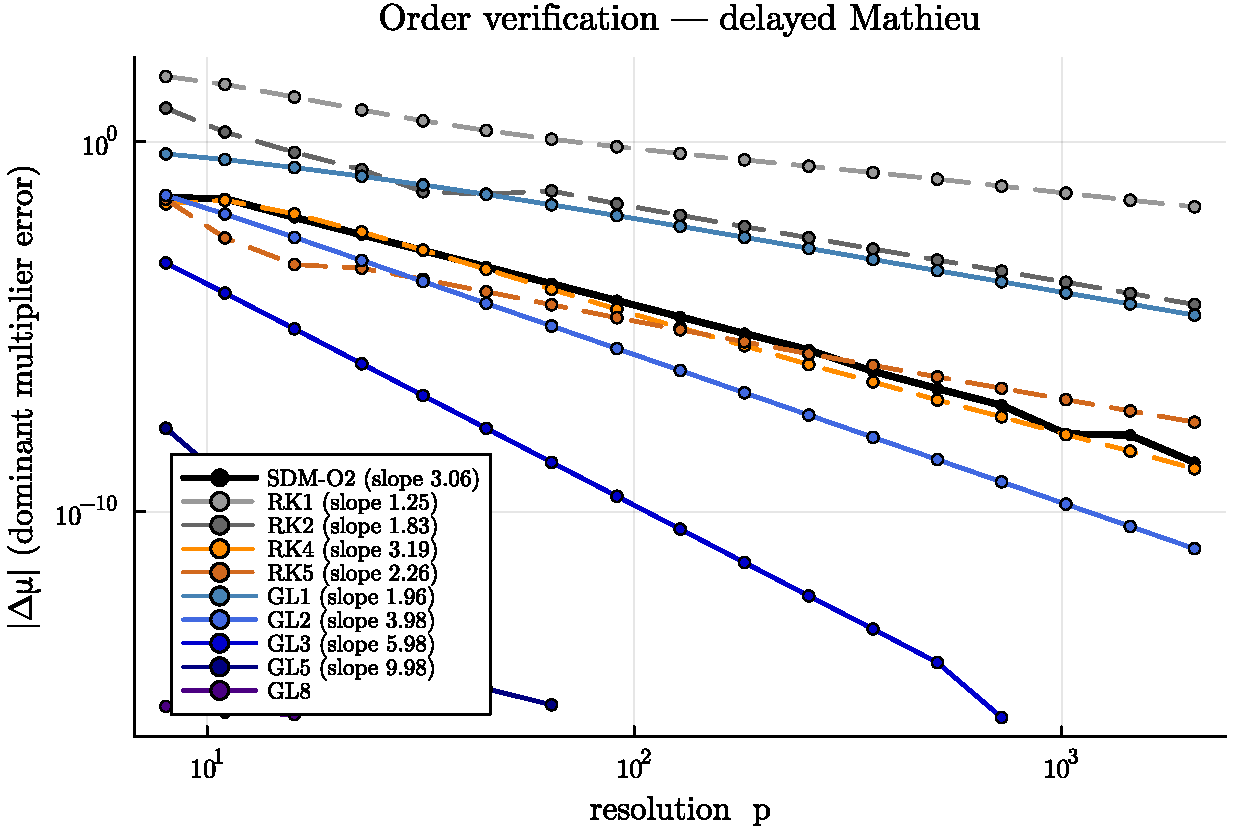
\includegraphics[width=\linewidth]{figures/order_verification.pdf}
  \caption{Order verification on the delayed Mathieu equation: eigenvalue
  error versus resolution $p$ (log--log), one curve per method, dashed lines
  showing fitted slopes. \TODOnum{regenerate from
  results/order\_verification\_mathieu.csv}}
  \label{fig:order}
\end{figure}

\subsection{Work--precision and time complexity}
\label{sec:wp}

\TODOnum{Figures: 4-panel work-precision per system; complexity plot with
mean$\pm1\sigma$ bands and fitted exponents $\approx 1.0$ for all MFCM
variants; SDM reference curve.}

\subsection{The accuracy--sparsity sweet spot}
\label{sec:sweetspot}

For a fixed relative accuracy target $\varepsilon$, sweeping the per-step
order $s$ while choosing the smallest resolution $p$ that reaches
$\varepsilon$ produces a U-shaped CPU-time curve: low orders need excessive
$p$, high orders pay cubically growing per-step fill,
$\mathrm{nnz}(\mathbf{\Phi}_\mathrm{L}) \sim p\,d^2 s^3$. A first-order
cost model, $\mathrm{cost} \propto p\,s^3$ with
$\varepsilon \propto (T/p)^{2s}$, predicts the optimum
\begin{equation}
  s^\ast \approx \tfrac{1}{6}\ln(1/\varepsilon),
  \label{eq:sweetspot}
\end{equation}
i.e.\ even a $10^{-12}$ accuracy target asks for only $s^\ast \approx 5$
Gauss stages --- moderate order, many steps. The measured optima
(\TODOnum{Mathieu: $s^\ast=\ldots$; beam: $s^\ast=\ldots$ at
$\varepsilon = 10^{-5},10^{-8},10^{-11}$}) confirm both the U-shape and its
logarithmic drift with $\varepsilon$, and the beam shifts the optimum to
lower order than the small Mathieu system, as predicted by the
$d^2$-scaling of the fill.

\subsection{Explicit versus implicit steps}
\label{sec:expl-impl}

\TODOnum{Overlay from work-precision data: explicit RK4/RK5 vs GL2/GL3;
regimes where the cheap triangular structure of explicit steps wins
wall-clock despite lower order, and where Gauss super-convergence wins
because far fewer points are needed.}

\subsection{Non-smoothness stress test}
\label{sec:nonsmooth}

With act-and-wait switching active, the beam's feedback matrix jumps at
$t = 0.8\,T$. When the switching instant falls on a grid node the full order
is retained; when it falls inside a step, all high-order methods collapse
towards low observed order near the switching-induced error floor
(\TODOnum{fitted slopes aligned vs off-grid for GL1/GL2/GL3}). Moderate
order with many steps is thus also the \emph{robust} choice for non-smooth
engineering systems --- reinforcing, not weakening, the sweet-spot message.

\section{Discussion: practical guidance}
\label{sec:discussion}

\TODOnum{Decision rule finalized after numbers: given dimension $d$,
resolution demand (period-to-delay ratio, coefficient smoothness) and target
accuracy, recommend Gauss stages $s \approx \max(2, \lceil \ln(1/\varepsilon)/6
\rceil)$ capped by the $d^2 s^3$ fill, explicit RK4 for very cheap
moderate-accuracy sweeps, and warn against single-step spectral mode for
$d \gtrsim 10$ or non-smooth coefficients.}

\section{Conclusion}
\label{sec:conclusion}

Once the stability analysis of time-periodic DDEs is written in
multiplication-free banded form, the per-step integrator is a free design
choice: Butcher-tableau residual blocks with continuous-extension delay
interpolation raise the convergence order to that of the chosen scheme, up to
Gauss super-convergence $2s$, while retaining $\mathcal{O}(p)$ complexity.
The two classical method families are the endpoints of one continuum ---
piecewise-constant semi-discretization at maximal sparsity and global
collocation at maximal per-step order --- and neither endpoint is optimal:
the CPU-time optimum sits at a problem-dependent sweet spot of moderate order
and many steps, drifting only logarithmically with the accuracy target and
towards lower order for larger system dimension and non-smooth coefficients.
This unifies and clarifies, rather than reinvents; the actionable outputs are
the sweet-spot guidance and the open-source \textsf{MFCM.jl} implementation.

\begin{acks}
\TODOnum{funding, computing acknowledgements}
\end{acks}

\begin{dci}
The author declares no conflict of interest.
\end{dci}

\appendix

\section{Model parameters}
\label{app:params}

\TODOnum{Full parameter tables for the four systems, copied from
benchmark/harness.jl definitions: Mathieu ($\delta=3$, $\varepsilon=0.2$,
$b_0=-0.15$, $a_1=0.1$, $\tau=T=2\pi$); seasonal ($a=1$, $b=1$, $\tau=2$,
$T=2\pi$); turning SSV ($k_w=0.2$, $\zeta=0.1$, $\Omega=0.3$,
$A_\mathrm{SSV}=0.1$, $N_T=10$); beam ($E=210$\,GPa, $A=10^{-4}$\,m$^2$,
$\rho=7800$\,kg/m$^3$, $L=100$\,m, $\eta=0.01$, $N=15$, $P=0.2$,
$\tau = 0.2\,L/c$, $T = 0.4\,L/c$, switch at $0.8\,T$).}

\section{Reproducibility}
\label{app:repro}

\TODOnum{Julia version, package versions, machine, BLAS threads = 1,
repository URL and commit hash; every figure regenerable by
\texttt{julia --project=benchmark benchmark/run\_all.jl} followed by
\texttt{make\_figures.jl}.}

\bibliographystyle{SageH}
\bibliography{references}

\end{document}
